\documentclass[8pt, twocolumn]{article}
\usepackage{amsmath}
\usepackage{graphicx}
\usepackage{float}
\usepackage[margin=0.75in]{geometry}

\author{Jaime Guerrero}
\title{Parallelization of Karatsuba's Algorithm using Cilk}
\date{\today}

\begin{document}

\maketitle

\section{Overview}
I provide a implementation of Karatsuba's multiplication algorithm that has
been parallelized with the Cilk extensions to C.  By taking a correct,
sequential version of the program, impressive speedups are possible with
minimal programmer effort.

\section{Background}
The grade-school multiplication algorithm we all learned is easy to understand
but not necessarily algorithmically efficient.  In particular, the naive
algorithm requires $O(n^2)$ operations, where $n$ is the number of bits being
multiplied.  Karatsuba's algorithm, in contrast, takes a divide-and-conquer
approach and only requires $O(n^{\log_2 3})$ operations.  This speedup is gained
by reducing the number of multiplications that must be done in
exchange for a few more additions.

Consider two binary multiplicands $U$ and $V$ that are powers of two.
Furthermore, let the subscript 1 denotes the high-order bits of a given
multiplicand and 2 the low-order bits.  The naive multiplication generates the
product
\begin{align}
   UV = U_1 V_1 2^{2n} + (U_1 V_2 + U_2 V_1)2^n + U_2 V_2.
\end{align}
To generate the product $UV$, four multiplications are required: $U_1V_1,
U_1V_2, U_2V_1$, and $U_2 V_2$.  The following modification of the
above equation is the inspiration for the algorithm and provides the speed increase:
\begin{align}
\begin{split}
UV = \quad & U_1 V_1 2^{2n} + \\ &[(U_1 + U_2)(V_1 + V_2) - U_1 V_1 - U_2 V_2]2^n + \\
     & U_2 V_2
\end{split}
\end{align}
In this form only three multiplications are needed: $U_iV_i$ and $(U_1 + U_2)(V_1 + V_2)$.

While Karatsuba's algorithm is easy to understand, a variety of faster
multiplication routines exist. The GNU Multiple Precision Arithmetic Library
(GMP) uses some of these routines in their own multiplication routines
\cite{gmp-mult}. By analyzing the multiplicand sizes, GMP chooses the most
appropriate multiplication routine for the job.  The speed of the algorithms is
further increased through the inclusion of highly optimized assembly code
\cite{gmp-home}.

The sequential C implementation of Karatsuba's algorithm included here was the
capstone project for Paul Purdom's \textit{Algorithm Design and Analysis} class
taken in Spring 2014.  The goals of this project were twofold: the first was to
have the fastest implementation possible when compared to other students in the
class and GMP.  The second goal was to carefully analyze an algorithm, given the
constraints of a machine's architecture.  With the help of Tim Zakian and
Spenser Bauman, the sequential version presented here was the fastest of that
semester.

\section{The Setup}
The GMP library is used to generate random bignums which are then multiplied by
both the implementation of Karatsuba's algorithm and GMP. GMP also provides
methods for comparing two bignums for equality. Thus, I was able to compare
Karatsuba's algorithm for both speed and correctness.

In the vein of most divide-and-conquer algorithms, Karatsuba is amenable to
parallelization.  Rather than waiting for sequential processes to work upon one
half of the input at a time, both haves can be worked upon in parallel, with
their answers combined at the end of the computation.

The programming model provided by Cilk was a natural choice for this project.
Cilk's fork-join approach to parallelism makes it easy to know where to place
calls to \texttt{cilk\_spawn} and \texttt{cilk\_sync}, and its provably
efficient work-stealing scheduler ensures that any parallelism speedup is not
sensitive to load-balancing and communication protocols \cite{leiserson}.  When
the original code was modified to run in parallel, only four lines were changed.
Three calls to \texttt{karatsuba()} were changed to \texttt{cilk\_spawn
karatsuba()}, and one \texttt{cilk\_sync()} was placed immediately afterward.
Furthermore, Cilk's C elision property ensures that changes to that those four
lines will maintain the original program's semantics, but (hopefully) just run
faster.

\section{Benchmarks}
\begin{figure}[t]
    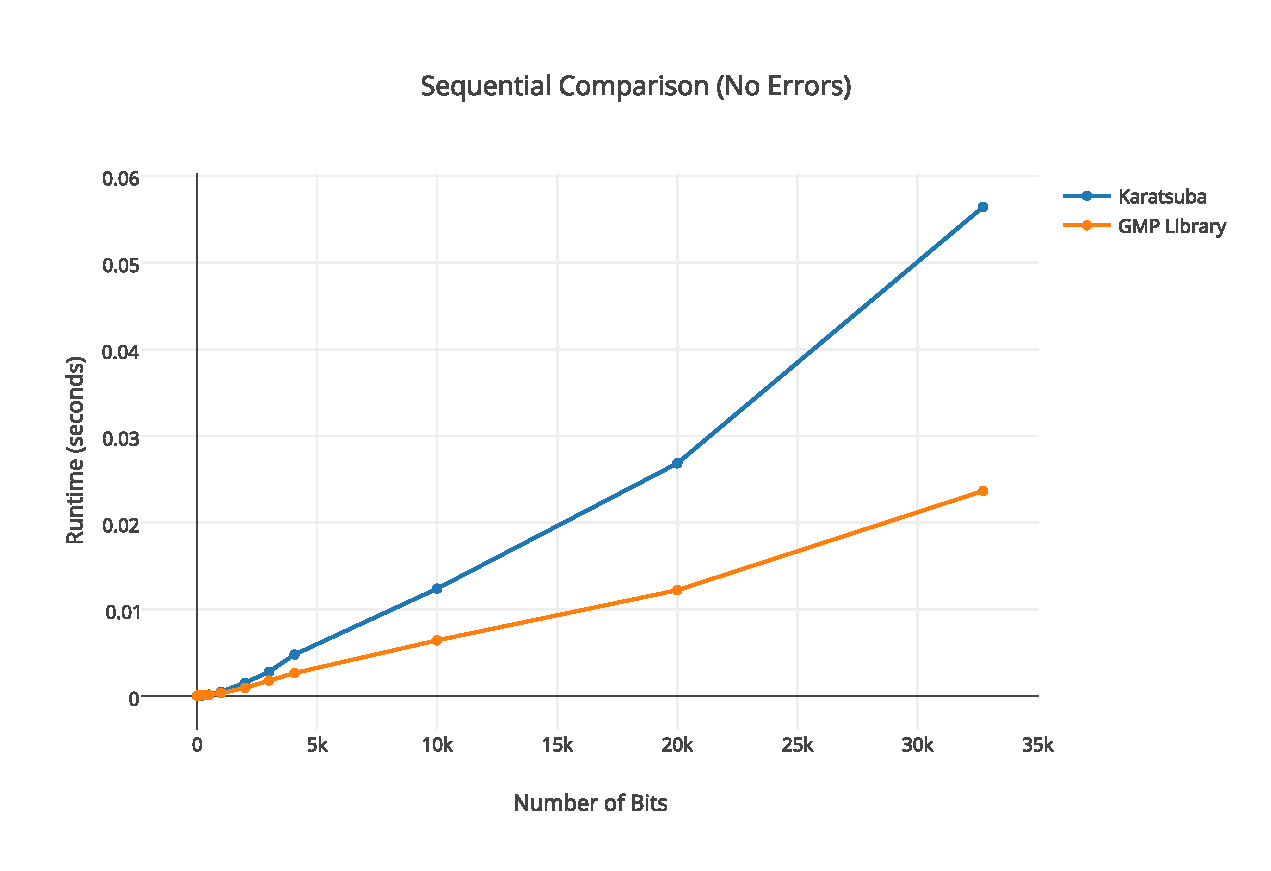
\includegraphics[scale=0.4]{sequential-error-free}
    \caption{Runtimes of sequential Karatsuba and GMP, wherein all Karatsuba answers
    are correct.}
    \label{fig:sequential-correct}
\end{figure}
All tests were run on ``Wolverine'', an 8-core, 64-bit machine running Red Hat
Linux version 2.6.32 with 16 GB of RAM.  Several optimizations were applied to
the sequential version of the code.  The most interesting are detailed below:
\begin{enumerate}
    \item \texttt{-march=native} switch: Allows for highly specialized compilation
          that is tuned to the machine's architecture.
    \item \texttt{-fomit-frame-pointer} switch: Provides an extra register when the
           frame-pointer does not need to be kept around.
    \item \texttt{-fdelete-null-pointer-checks} switch:  Do not check for null
          pointers.
    \item \texttt{-fif-conversion2} switch: Per the online GCC manual, ``Transforms
          conditional jumps into branch-less equivalents''.
    \item \texttt{((flatten))} pragma: inline as much of a function's body as
          possible.
    \item \texttt{((nothrow))} pragma: note that a function will not throw an
          exception.
\end{enumerate}

Regardless of the number of optimizations enabled, poorly structured code will
still run slowly. Consequently, the code minimizes minimize memory
allocation/deallocation and groups together repeated function calls.

The main program driver runs both the GMP multiplication routine and Karatsuba's
algorithm 100 times; the running time of both (in seconds) are presented here.
Figure \ref{fig:sequential-correct} shows the benchmarks for the very first
implementation from Purdom's class. This initial sequential program was
originally tested on numbers not exceeding 32736 bits, and all answers were
correct.

For the sake of fully exploring the implementation, I experimented with larger inputs.
 At around two-hundred thousand bits, the sequential Karatsuba
begins to produce wrong answers, while the parallel version produces wrong
answers at four million bits.  To that end, the only measurements presented here
were those that were correct.  The cause for these wrong answers is unknown.  It
was originally believed to be a matter of freeing all allocated memory; this
remedied all incorrect answers in the parallel version for small inputs,
though did not scale as expected. \newline
\begin{figure}[t]
    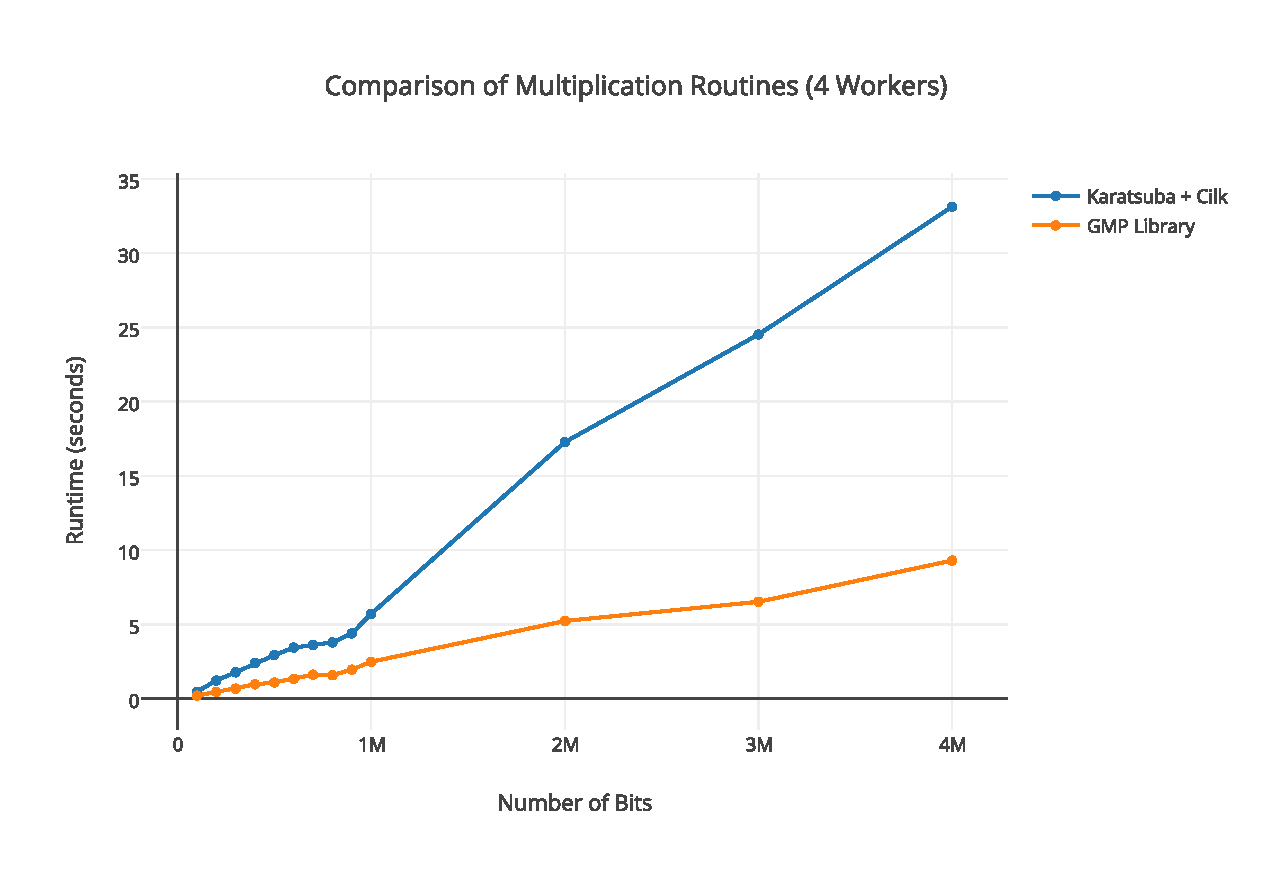
\includegraphics[scale=0.4]{4-workers}
    \caption{Comparison of GMP with 4 Cilk workers.}
    \label{fig:4-workers}
\end{figure}
\begin{figure}[t]
    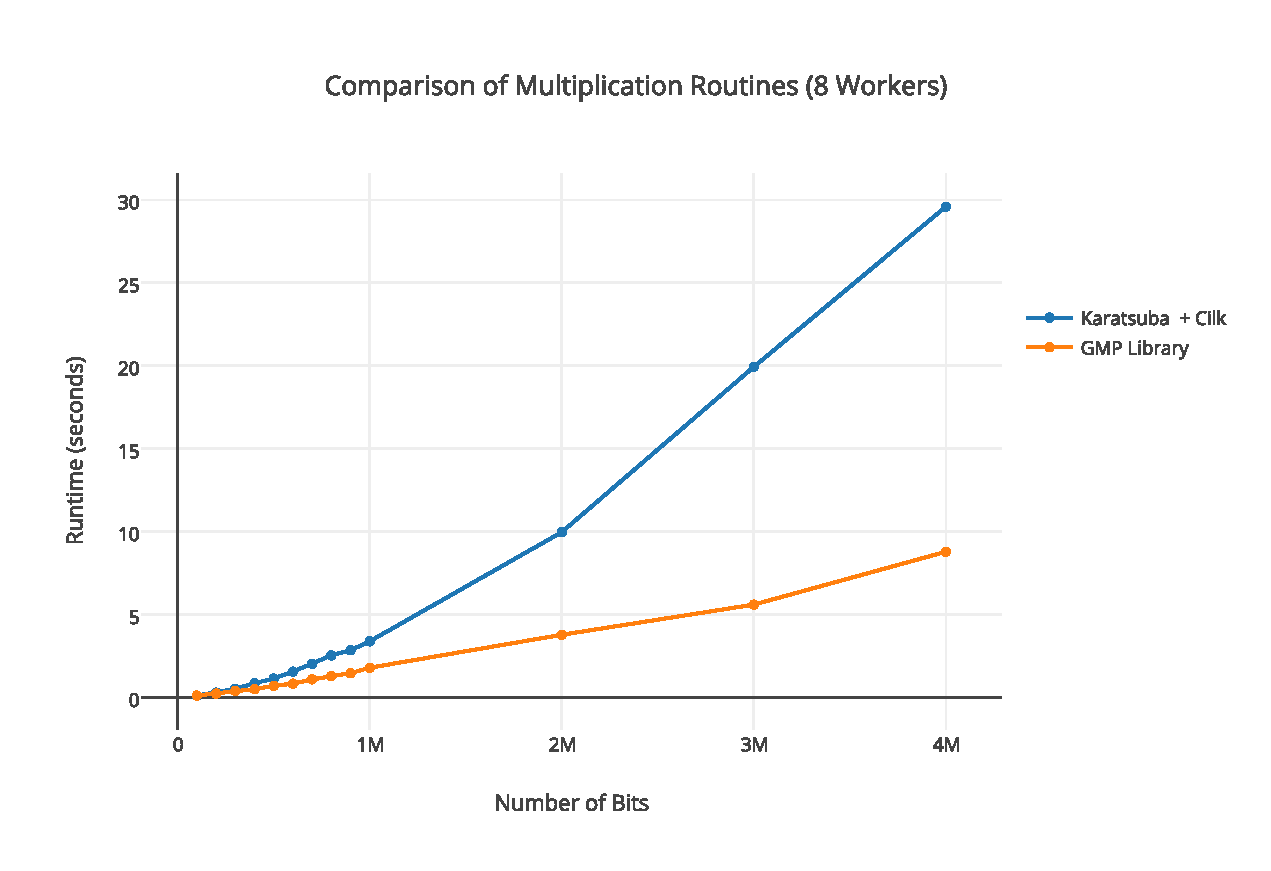
\includegraphics[scale=0.4]{8-workers}
    \caption{Comparison of GMP with 8 Cilk workers.}
    \label{fig:8-workers}
\end{figure}
Since the 8 and 16 workers versions are so similar in their runtimes, I have
only included the 8 worker data for the sake of space.  Both Figure
\ref{fig:4-workers} and Figure \ref{fig:8-workers} show that the parallel
algorithm is competitive with the GMP routine up until around one million
digits.  The dropoff of Karatsuba is most pronounced in the 4-worker version.
Most notable is the speedup Cilk provides when compared to the sequential
version.  Figure \ref{fig:parallel-vs-sequential} demonstrates that Cilk is
comparable to sequential C for small inputs, and its gains are appreciable for
large inputs.  GMP has the benefit of hundreds of developer hours and more
sophisticated multiplication routines, and it is clearly the superior choice
when speed is the main requirement.  However, Cilk provides a solid performance
improvement and a low barrier to entry that makes it an attractive tool for the
average programmer.
\begin{figure}[H]
    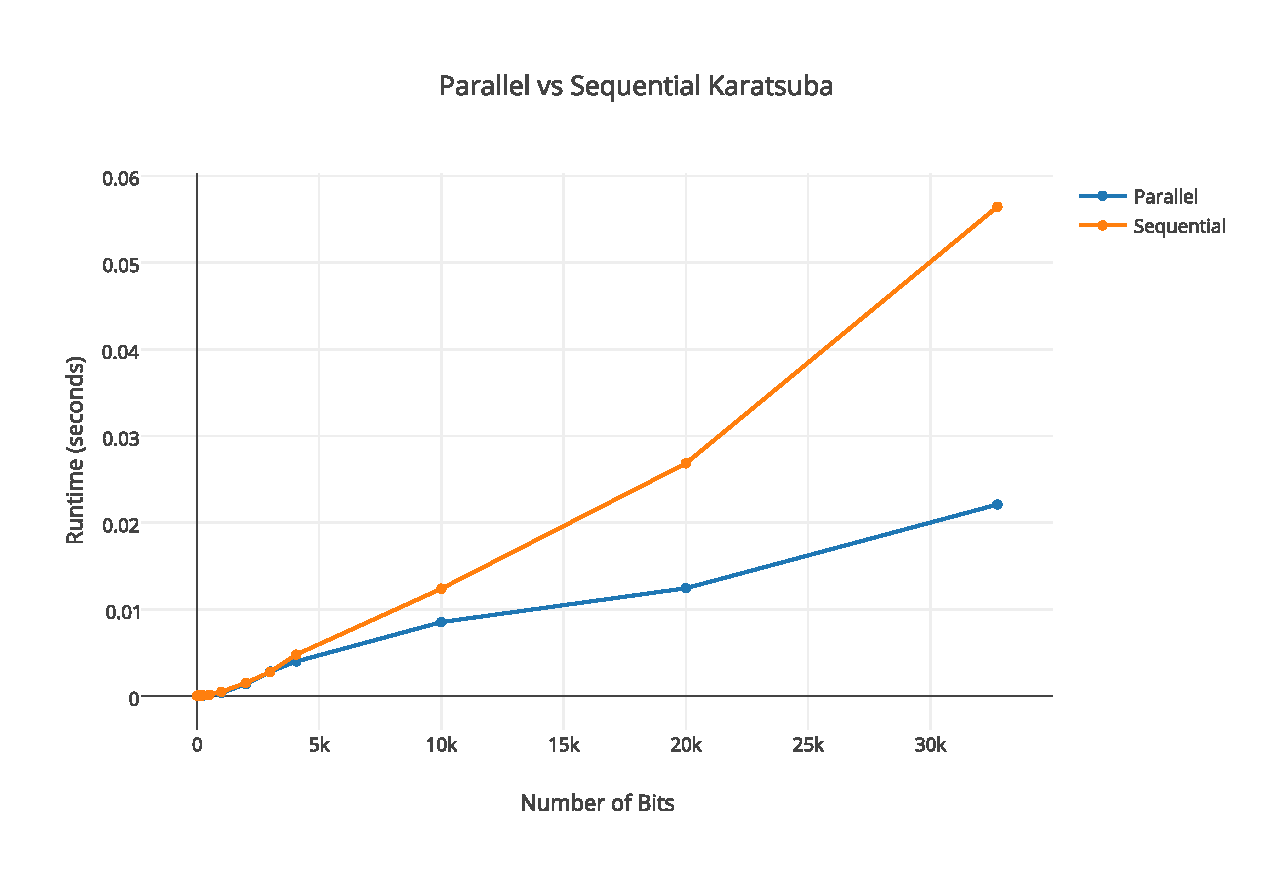
\includegraphics[scale=0.4]{parallel-vs-sequential}
    \caption{Parallel performance in comparison to sequential implementation.}
    \label{fig:parallel-vs-sequential}
\end{figure}

\begin{thebibliography}{9}

\bibitem{gmp-mult}
\emph{GMP Multiplication Algorithms},
https://gmplib.org/manual/Multiplication-Algorithms.html,
June 21, 2015.

\bibitem{gmp-home}
\emph{The GNU Multiple Precision Arithmetic Library},
https://gmplib.org,
June 21, 2015.

\bibitem{leiserson}
\emph{Programming Parallel Applications in Cilk},
SIAM News,
Volume 31, Number 4,
May 1998.

\end{thebibliography}
\clearpage
\onecolumn
\begin{appendix}
\section{Karatsuba's Algorithm}
The Karatsuba multiplication algorithm as outlined by Purdom and Brown.

Input: the $2n$-bit number $U = U_1 2^n + U_2$ where $0 \leq U_1 < 2^n$ and $0
\leq U_2 < 2^n$, and the $2n$-bit number $V=V_1 2^n + V_2$ where $0 \leq V_n
< V^n$.

Output: The product $UV$ represented by $UV = W_1 2^{3n} + W_2 W^{2n} + W_3 2^n + W_4$.

\begin{enumerate}
    \item Set $T_1       := U_1 + U_2$
    \item Set $T_2       := V_1 + V_2$
    \item Set $W_3       := T_1 T_2$
    \item Set $W_2       := U_1 V_1$
    \item Set $W_4       := U_2 V_2$
    \item Set $TempDiff  := W_3 - W_2$
    \item Set $TotalDiff := TempDiff - W_4$
    \item Set $Carry     := \lfloor W_4 / 2^n \rfloor$
    \item $W_4            = W_4 \mod 2^n$
    \item Set $\hat{W_3} := TotalDiff + Carry$
    \item Set $\bar{C}   := \lfloor \hat{W_3} / 2^n \rfloor$
    \item $W_3            = \hat{W_3} \mod 2^n$
    \item Set $\hat{W_2} := W_2 + \bar{C}$
    \item $W_1            = \lfloor \hat{W_2} / 2^n \rfloor$
    \item $W_2            = \hat{W_2} \mod 2^n$
\end{enumerate}
\end{appendix}

\end{document}
